\documentclass[11pt]{article}
\usepackage[utf8]{inputenc}
\usepackage{graphicx}
\usepackage[left=1.8cm, right=1.8cm, top=2cm, bottom=1.8cm]{geometry}
\usepackage{tabularx}
\usepackage{pbox}
\usepackage{physics}
\usepackage{booktabs}
\usepackage{fancyhdr}
\usepackage{enumitem}
\usepackage{multirow}
\usepackage{ctable}
\usepackage[medium]{titlesec}
\setlength{\textfloatsep}{-10pt}
\pagestyle{fancy}


\title{Analyse Numérique : Devoir 1}
\author{Valentin Lemaire}
\date{28 Octobre 2019}

\begin{document}
\rhead{Valentin Lemaire - 16341700}
\lhead{Devoir 2 : Factorisations LU et QR}

\section{Factorisation LU}
\vspace{-8pt}
L'algorithme implémenté dans la fonction \texttt{LU(A)} est assez simple. Il s'agit d'une simple vectorisation de la fonction \texttt{LU\_slow(A)} qui elle est l'implémentation classique de l'algorithme LU avec 3 boucles for. Dans la version améliorée, au lieu de copier les lignes permutées, on utilise simplement le vecteur P pour faire les appels à A pour pouvoir tenir compte des permutations sans devoir recopier les lignes. 
\vspace{-5pt}
\paragraph{Déterminant} Puisque $PA = LU$, $A = PLU$ (P est toujours inversible et $P^{-1} = P$) et que $det(AB) = det(A)det(B)$, on a : $det(A) = det(P)det(L)det(U)$. On sait que $det(P) = (-1)^n$ où $n$ est le nombre de permutations effectuées sur la matrice, que $det(L) = 1$ puisque c'est une matrice triangulaire dont tous les éléments diagonaux sont 1 et que $det(U)$ vaut le produit de tous ses éléments diagonaux (matrice triangulaire). Dès lors, on a : $det(A) = (-1)^n det(U)$. Puisqu'on a enregistré le nombre de permutations dans l'algorithme LU dans le $N+1^{ème}$ élément de P, le déterminant est obtenu très facilement.  
\vspace{-5pt}
\paragraph{Inverse} Puisque $A = PLU$, et qu'on sait que l'inverse de $A$ est la matrice $A^{-1}$ telle que $AA^{-1} = I$, on a $PLU A^{-1} = I$ et donc, $LU A^{-1} = PI$. Dès lors, on trouve facilement que pour chaque colonne $a^{-1}_i$ de la matrice $A^{-1}$ : $LU a^{-1}_i = (PI)_i$. Comme $L$ et $U$ sont des matrices triangulaires, ce système est résolu très rapidement et on peut trouver tous les vecteurs colonnes de la matrice inverse $A^{-1}$ de cette manière.
\vspace{-5pt}
\paragraph{ILU(0)} L'algorithme ILU(0) a été implémenté de trois manières : \texttt{ILU0\_slow(A)} qui est la version lente de l'algorithme, \texttt{ILU0\_always\_pivot(A)} qui est la version vectorisée de ce même algorithme et \texttt{ILU0(A)} qui est la même que la précédente avec une petite différence. Les deux boucles for imbriquées dans la grande boucle ont été retirées et on ne fait le calcul que sur les éléments non-nuls en récupérant leurs indices non-nuls grâce à la fonction \texttt{nonzero} de numpy. Cette version de l'agorithme fonctionne dans 2 régimes sur 4 (pas en dynamique ni en stationnaire) car à un certain moment, il ne trouve plus de pivot non-nul. Dès lors, la fonction \texttt{ILU0(A)} ne cherche le plus grand élément de la colonne pour en faire le pivot que si le pivot "naturel" est nul. Ainsi, l'algorithme marche dans les 4 régimes et en plus est un peu plus rapide.
 \vspace{-5pt}
\paragraph{Solveur LU} La fonction \texttt{LUsolve(A, b, P)} tire profit du caractère triangulaire des matrices L et U et résoud successivement deux systèmes linéaires : $Ly = Pb$ et $Ux = y$ en tirant du fait que les matrices $L$ et $U$ sont triangulaires. La résolution est donc presque immédiate.
\vspace{-10pt}
\section{Factorisation QR}
\vspace{-8pt}
L'algorithme de factorisation QR (en particulier, celui de Gram-Schmidt) a été implémenté de 3 manières différentes. Une première fois dans \texttt{QR\_slow(A)} de manière naïve avec trois boucles for, une seconde fois dans \texttt{QR\_columns(A)} qui est la version complètement vectorisée de la fonction précédente. Et enfin, \texttt{QR(A)} qui transpose A au début pour qu'on puisse effectuer toutes les opérations sur les lignes plutôt que sur les colonnes (permet les opérations par blocs) ce qui rend le code plus rapide. Dans cette version, on a égaleemnt enregistré Q dans A plutôt que de créer une nouvelle matrice par souci de mémoire.
\vspace{-5pt}
\paragraph{Solveur QR} Le solveur QR (implémenté dans \texttt{QRsolve(A, b)} prend en argument une matrice $A$ et un vecteur $b$ et commence par appeler \texttt{QR(A)} pour réaliser la factorisation QR, et ensuite, résoud le système (au sens des moindres carrés si le système est surdéterminé) $QRx = b$ ou encore $Rx = Q^* b$ en tirant profit du fait que la matrice $R$ est une matrice triangulaire supérieure.
\vspace{-10pt}
\subsection*{Analyse}
\vspace{-5pt}
\subsection{Complexité temporelle}
\vspace{-5pt}
\paragraph{Solveur LU} Comme vu au cours, le nombre d'opérations de l'algorithme LU est proportionel à $n^3/3$ (sans compter les termes de degré inférieur) et donc son ordre est : $\matcal{O}(n^3)$. Cependant, si on optimise (comme cela a été décrit ci-dessus) et qu'on considère que les opérations sur les lignes d'une matrices comme étant à temps constant, on voit que toutes les opérations dans la boucle sont en $\matcal{O}(n)$ et donc l'ordre de LU vectorisé devient $\matcal{O}(n^2)$. La partie résolution du système matriciel, en vectorisé prend quant à elle, un temps négligeable ($\matcal{O}(n)$) par rapport à la décomposition.
\vspace{-5pt}
\paragraph{Solveur QR} Le nombre d'opérations de la décomposition QR est quant à lui proportionnel à $n^3$ (à nouveau sans compter les termes de degrés inférieurs) et son ordre est donc $\matcal{O}(n^3)$. A nouveau en vectorisant (et en transposant la matrice pour pouvoir faire les opérations sur les lignes plutot que les colonnes), on peut considérer que ces dites opérations sur les lignes se font en temps constant et donc l'ordre de la décomposition QR devient $\matcal{O}(n^2)$
\begin{figure}
    \begin{minipage}{0.45\linewidth}
    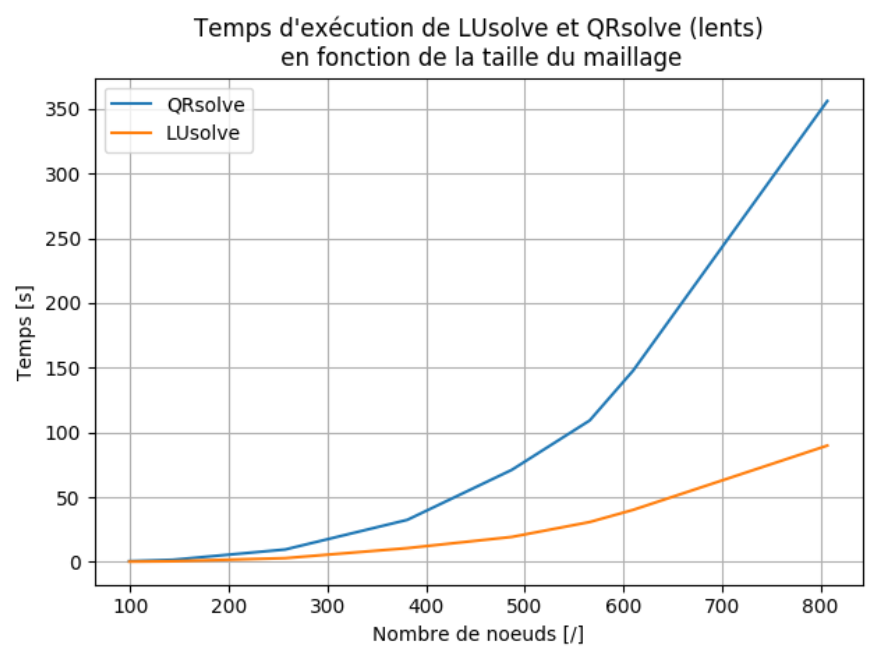
\includegraphics[width=\textwidth]{slow.png}
    \label{slow}
    \end{minipage}\hfill \begin{minipage}{0.46 \linewidth}
    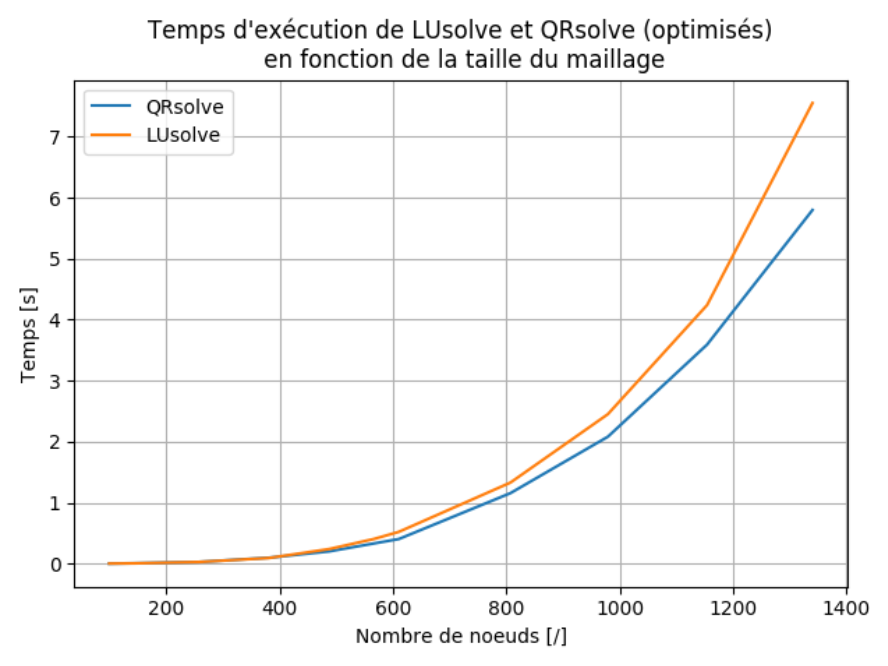
\includegraphics[width=\textwidth]{opt.png}
    \label{opt}
    \end{minipage}\hfill 
\end{figure}

Sur les graphes ci-dessus, on voit effectivement que pour les versions lentes (avec 3 boucles), QRsolve prend 3 fois plus de temps que LUsolve. C'est ce à quoi on s'attendait. En revanche, en versions optimisées, QRsolve semble un peu plus rapide que LUsolve bien que tous les deux du même ordre de grandeur (ils sont en effet tous les deux de l'odre $\matclal{O}(n^2)$).\footnote{Ne connaissant pas les détails de l'implémentation des opérations par blocs en python, je ne peux analyser plus que ça la différence de temps entre les deux implémentations (i.e. comparer le nombre d'opérations)}

\vspace{-10pt}
\subsection{Précision et temps d'exécutions de LUsolve et QRsolve}
\vspace{-8pt}
Dans le tableau \ref{solvercomp} nous présentons, pour les 4 régimes et sur un maillage de 1033 noeuds les temps d'exécutions des deux fonctions LUsolve et QRsolve (en tenant compte du temps pour nécessaire pour la factorisation), la précision de la solution obtenue (calculée avec : $\frac{||Ax-b||_2}{ ||b||_2}$) et la comparons avec le solveur de numpy : \texttt{np.linalg.solve(A,b)}. Bien évidemment, les temps dépendront d'une exécution à l'autre. Ils sont là pour donner une idée de l'ordre de grandeur. 

\begin{table} [h]
\centering
\begin{tabular}{|c|c||c|c|c|}
    \hline
     \multicolumn{2}{|c||}{}   & \textbf{Solveur numpy} & \textbf{Solveur LU} & \textbf{Solveur QR} \\
    \hline
    \multirow{2}{*}{\textbf{Statique} ($v=0$, $f=0$)} & \textbf{Temps d'exécution} [s] & 0.04644 & 3.032 & 2.577\\ \cline{2-5}
    & \textbf{Précision} [/] & $1.93 \cdot 10^{-14}$ & $6.22 \cdot 10^{-14}$  &  $5.57 \cdot 10^{-14}$\\
    \hline
    \multirow{2}{*}{\textbf{Stationnaire} ($v \neq 0$, $f=0$)} & \textbf{Temps d'exécution} [s] & 0.04551 & 3.026 & 2.603 \\ \cline{2-5}
    & \textbf{Précision} [/] & $1.04 \cdot 10^{-14}$ & $3.36\cdot 10^{-14}$& $4.12 \cdot 10^{-14}$\\
    \hline
    \multirow{2}{*}{\textbf{Harmonique} ($v=0$, $f\neq 0$)} & \textbf{Temps d'exécution} [s] & 0.04290 & 2.824 & 2.521\\ \cline{2-5}
    & \textbf{Précision} [/] & $2.25 \cdot 10^{-14}$ & $4.05\cdot 10^{-14}$ & $5.42 \cdot 10^{-14}$\\
    \hline
    \multirow{2}{*}{\textbf{Dynamique} ($v \neq 0$, $f \neq 0$)} & \textbf{Temps d'exécution} [s] & 0.03859 & 2.876 & 2.495\\ \cline{2-5}
    & \textbf{Précision} [/] & $1.3120 \cdot 10^{-14}$ & $3.55\cdot 10^{-14}$ & $4.00 \cdot 10^{-14}$\\
    \hline
\end{tabular}
\caption{Comparaisons des solveurs pour les 4 régimes}
\label{solvercomp}
\end{table}
On voit, sans surprises, que le solveur numpy est le plus rapide et le plus précis. Quant aux deux autres solveurs, on voit que LU est de manière générale un peu plus précis (sauf dans le cas statique) mais la précision reste dans le même ordre de grandeur (qui est le même que celui du solveur numpy également) mais la résolution du système par factorisation QR est légèrement plus rapide que la résolution avec factorisation LU. 
\vspace{-10pt}
\subsection{Conditionnement de $A$ et $M^{-1}A$}
\vspace{-8pt}

Le tableau \ref{condcomp} montre les differents nombres de conditionnement dans les 4 régimes pour la matrice $A$ ($\kappa_A$) et pour la matrice $M^{-1}A$ ($\kappa_{M^{-1}A}$) où $M$ est la décomposition LU de A avec l'algorithme ILU(0). L'utilité principale de cette matrice $M$ qui résulte de l'approximation de la décomposition LU de la matrice $A$ est de préconditionner un système. En effet, le temps nécessaire pour résoudre un système $Ax = b$ de manière itérative est proportionnel à $\sqrt{\kappa_A}$ donc si $A$ est mal conditionnée, la méthode sera lente. Par contre, si on transforme le système en $M^{-1}A x = M^{-1}b$ avec une matrice $M$ telle que le conditionnement de $M^{-1}A$ est meilleur que celui de $A$, la méthode convergera plus vite. La décomposition ILU(0) donne une telle matrice. \\
\begin{table}[h!]
    \centering
    \begin{tabular}{|c|c|c|c|c|}
        \hline
         & Statique & Stationnaire & Harmonique & Dynamique \\
         \hline
         $\kappa_A$ [/] & 1330.2 & 4157.7 & 1320.9 & 4191.0 \\
         \hline
        $\kappa_{M^{-1}A}$ [/] & 54.785 & 86.196 & 46.494 & 88.211 \\
         \hline
    \end{tabular}
    \caption{Nombre de conditionnement de $A$ et $M^{-1}A$ dans les 4 régimes}
    \label{condcomp}
\end{table}
Si on observe les valeurs du tableau, on voit effectivement que le conditionnemnet de $M^{-1}A$ est meilleur que celui de $A$ et ce, dans tous les régimes. La décomposition ILU(0) de $A$ fournit donc bien un bon point de départ pour une méthode de résolution itérative (gradients conjugués par exemple). Remarquons que les régimes pour lesquels $A$  était très mal conditionnée (stationnaire et dynamique) on un nombre de conditionnement $\kappa_{M^{-1}A}$ plus grand que les autres (statique et harmonique)
\end{document}